\justifying 

This thesis addressed several questions regarding solar flares and their effects on the local plasma environment. We also describe multiple initial preparatory analyses we carried out for the design and calibration for {\suit}. We first describe the analysis we carried out with the simulated spacecraft jitter data provided by the ISRO URSC team to quantify the RMS jitter as a function of exposure time. Following this, we describe the throughput model of {\suit}, and using the model, how we carry out the photometric and spectral validation of the payload in the lab. We also describe how this method was used to choose the science filters to be mounted on {\suit}. Subsequently, we describe the on-orbit stellar calibration plan of {\suit} using Sirius-A as a calibration source yet to be carried out. We then describe the forward model pipeline we set up to create mock {\suit} observations to characterize the imaging performance and the effects of the instrument PSF on the imaging. Following this, we use IRIS \ion{Mg}{2} data to investigate the effects of Solar flares on the local plasma environment. We describe how similar observations can be used to regularly monitor the similar effects from {\suit} NB3 and NB4 observations. We then move on to estimating thermal energies in two solar flares. We use DEM analysis with AIA, XRT and SUVI data to estimate the thermal energy of these flares as a function of time. We describe a method to use stereoscopic observations from AIA and {\it STEREO-A} data to accurately determine the flare arcade volume as a function of time. Finally, we describe the first flares observed by {\suit}. The main results of this thesis can be summarised as follows:

%%%%%%%%%%%%%%%%%%%
\begin{enumerate}
    \item The {\suit} payload has two main moving components {\it i.e.}, the shutter door and the filter wheel. We used a Fourier filtering method to isolate the movement with timescale $<$ 2 ms. 2 ms is relevant as that is the maximum permissible exposure time for {\suit}. We find that the RMS and average jitter in the worst possible case {\it i.e.}, when both shutter and FW are moving without any compensation is an order of magnitude smaller than 0.7{\arcsec}, the pixel size of {\suit}. So. it is safe to assume that the jitter would not affect the {\suit} imaging. 
    \item  We use the throughput model to describe how the photometric and spectral validation was carried out on ground, and how the science filters to be mounted on the payload were chosen. Our findings show that the measured data counts per second generally agree within a 20\% margin with those predicted by the throughput model (as detailed in Tab.~\ref{tab:throughput})), with the exception of NB07. A potential cause for this discrepancy is the use of SOLSPEC data for modeling throughput beyond 310 nm, while SOLSTICE data is used for wavelengths below this threshold. It is important to note that SOLSPEC data has a resolution of 0.05 nm, whereas SOLSTICE data offers a finer resolution of 0.025 nm. As a result, the lower resolution of SOLSPEC data reduces the accuracy of the modeled data counts for filters operating beyond 310 nm.
    
    \item We present the spectral validation results for all filter combinations with transmission bandpasses above 250 nm in Fig.~\ref{fig:sepc_calib}. In this figure, the x and y error bars represent the wavelength bins corresponding to the input slit size and the Poisson uncertainty of the measured ADC counts, respectively. The plots indicate that the measured shape of the instrument's spectral response closely matches the modeled spectral response for all filter combinations with transmission bandpasses above 250 nm.

    The spectral characterization for the NB08 filter could not be completed due to strong ghost reflections near the central patch. These reflections are caused by the absence of a relative tilt between the two stacked filters that create the NB08 bandpass, unlike other filters. As a result, the ghost reflections interfere with the estimation of ensquared energy across the transmission bandpass, compromising the spectral validation for this filter.

    \item We present the forward modelling pipeline setup which would enable us to create mock {\suit} observations from existing MHD simulations using the measured optical response of various components. This can be beneficial in constraining various model parameters by comparing the mock observations with real observations from {\suit}. Using the setup, existing observations from IRIS and measured PSFs we present the imaging performance of {\suit} discussing how various features are observed via {\suit}. We also present the initial deconvolution algorithm designed for deconvolving {\suit} observations and how it restores the observations.

    \item The ratios of \ion{Mg}{2} h and k ratios change during the evolution of flares. Limited by the single flares of C, M and X-class flare we observed, we see significant change only in the M and C class flare. The ratio increases at the onset of the flare, reaching the peak at the impulsive phase and sharply declining afterwards dropping below the pre-flare levels in the decay phase. The variation can be explained by localized heating and chromospheric evaporation in the impulsive phase, and condensation and down flow in decay phase. However this is speculative as we did not see the effects in X-class flare. Our findings indicate that the \ion{Mg}{2} k to h line intensity ratios fluctuate during flares. As shown in Figs. \ref{fig:optical_dep_ev_m},\ref{fig:align_raster_flare2} (right panel), and \ref{fig:optical_dep_ev_c}, the line intensity ratios remain consistent across varying magnetic field strengths, from weak to strong. This consistency suggests that the magnetic field influences both the Mg II k and h lines similarly, causing these effects to cancel out when the ratios are calculated.
    
    \item The estimation of thermal energy in solar flares depends significantly on the volume estimation. There were existing studies \citep{hilarie05} which already eluded the same. We propose a method with existing tools using stereoscopic observations from AIA and {\it STEREO-A}, to estimate the volume of the flaring arcade as a function of time. This demonstrates that the uncertainty in the volume estimation can lead to significantly overestimate the thermal output of the flare in the impulsive phase and the peak of the flare. Our method of estimating the thermal energy from imaging observations using DEM analysis also enables us to quantify the thermal output of various parts of the flares {\it e.g.} flare arcade, fan etc. separately. Using this, we showed that the fan of the limb event $\mathrm{29^{th}~November}$, 2020 was cooling at a different rate compared to the loops. This indicates that a distinct heating mechanism is at play in the fan which different from the loops, as described in various other studies (e.g. SADs \citep{reeves17}, plasma flow turbulence \citep{xie23}) via different methods.

    \item The first flare observations from {\suit} give us chromospheric diagnostics in various chromospheric and transition region lines. In this thesis, we discuss {\suit} observations of two limb flares and an on-disk flare. The results can be summarised as follows:
    %%%%%%%%%%%
    \begin{itemize}[label=\ding{226}]
        \item {\bf 22 Feb, 2024:} The on-disk flare shows umbral bright flare kernels in NB2 (blue wing of \ion{Mg}{2} window) and NB5 (red wing of \ion{Mg}{2} window). The flare brightening is co-temporal with HXR from STIX observations in NB3 (\ion{Mg}{2} k), NB4 (\ion{Mg}{2} h), and NB8 (\ion{Ca}{2} h). The bright kernels peak in intensity slightly later compared to the transition region lines {\it i.e.} \ion{Mg}{2} k \& h, \ion{Ca}{2} h. We also analyse the XSM spectra to find an excess in the Fe $\sim$ 6.5 keV complex. This excess can not be explained by multi-thermal plasma and satellite lines unaccounted in the fitting \citep{mithun22}. We also find that the excess component peaks in-between the SXR and HXR and corelates well with the SXR flux $>$ 7.12 keV. 
        
        \cite{kowalski19} observed umbral brightening kernels from another X-class flare. The {\it IRIS} raster scans in the 2832 {\AA} window revealed that the brightening was arising due to several \ion{Fe}{2} lines, which is usually in absorption, going into emission. They attributed photospheric heating as the reason for this. Similar observations of photospheric metallic lines going into emission was made by \cite{heinzel14,kleint17}. Due to the co-temporal nature of the NB2 and NB5 brightening with the Fe excess observed in XSM eludes that both of these are driven by the same process. The HXR flux from peak happens earlier, implying that the origin of umbral brightening kernels are not driven by the electron and/or ion beams from the coronal reconnection site. The co-temporal nature of the $>$ 7.12 keV SXR flux implies that this is what drives the formation of the umbral bright kernels as well as the excess in the Fe line observed by XSM. Fe K$\alpha$ fluorescence emission has been reported to exhibit similar characteristics as the excess observed by XSM \citep{doscheck71,tanaka84,phillips12,parmar84}. We believe this is direct observational evidence at photospheric heights, lower than the chromospheric condensation which was suspected to be the source of photospheric heating in \citep{kowalski19}. The flaring soft X-ray $>$ 7.12 keV photoionizes the ambient Fe present at photospheric heights, giving rise to plethora of \ion{Fe}{2} lines resulting in several electronic transitions between various vacated atomic levels. This gives rise to the characteristic K$\alpha$ emission excess observed. This provides us with important metallic lines arising from photospheric heights that can be important diagnostic for characterising solar flare models.
        
        \item {\bf 31 Dec, 2023:} The X5 flare exhibited an off-limb ejection in NB4 (\ion{Mg}{2} h) which was also observed in multiple AIA channels. We found that the ejecta observed in NB4 was cospatial with the structure observed in AIA 1600 {\AA} and 171 {\AA}. From DEM analysis we find that this region is part of an ejected loop that is denser and cooler compared to the rest of the structure. This might be a line of sight effect. This material is then ejected accelerating as it travels radially outwards. We find that the velocities calculated from AIA 1600 {\AA} and {\suit} NB4 observations are consistent with each other. From AIA 1600 {\AA} observations and STIX HXR light curves, we find that the accelerated ejection of the material is consistent with secondary reconnection at coronal altitudes and multiple ejection from the same active region. 
        
        \item {\bf 27 May, 2024:} The X2.9 flare was accompanied by a large prominence ejection followed by the rising flare arcades. The flare arcades have a cusp shape which are usually observed in homologous flares. For this flare we see post flare loops clearly in NB3, NB4 and NB8. Interestingly the loops are brighter in these lines just below the fan. From DEM analysis this region appears denser and cooler compared to the rest of the post flare loops. We find that a prominence was present in between the flare , which erupted launching colder material into the loops. Thus the loops appear brighter in the Mg and Ca lines. 
    \end{itemize}
    %%%%%%%%%%%
 
\end{enumerate}
%%%%%%%%%%%%%%%%%%%

The overarching progression of this thesis, starts from various preparatory analysis carried out for {\suit}. These studies helped us in realising several aspects of {\suit} in timely manner. Then we describe a mock observation pipeline setup for {\suit} observations which would allow us existing simulations with observations. Then the thesis delves into various flare observations, from existing observatories in anticipation of {\suit}, and later on, after successful launch and L1 insertion, observations from {\suit} which gives us unique perspective into solar flares and their effects in transition region and beyond. The results of this thesis raises various pressing questions,

\noindent
{\bf Why was changes in \ion{Mg}{2} k to h line intensity ratio not observed in the X-class flare?} We observed the correlated change in the M and C class flare, which can be explained via localised heating evaporation in preflare phase and condensation in the decay phase. But this still needs to be verified with a larger sample of flares. The few X-class flares we have observed with {\suit} show the correlated changes in NB3 (\ion{Mg}{2} k) and NB4 (\ion{Mg}{2} h) line intensity ratio. This raises two distinct possibilities:

    %%%%%%%%%%%
    \begin{itemize}[label=\ding{226}]
        \item There is a possibility that the change was not observed for the X class flare, simply due to the cadence limitations of IRIS raster scan, along with which regions of the flare arcade is being scanned by IRIS because it is well known that the \ion{Mg}{2} profiles vary significantly in shape and spatially within the flaring region \citep{panos18,dalda23}.
        \item The other, more interesting possibility is that in some of the events depending on the "impulsiveness" of the event, there might be different degrees of ionisation at play at the chromosphere. This also might indicate a different energy release mechanism during the preflare and impulsive phase.
        \item One of the crucial tools in this regard would be finding correlations between {\it IRIS} and {\suit} observations. {\it IRIS} has been taking regular planned observations for {\suit} in QS and AR. One of the studies we will conduct immediately, is correlate {\it IRIS} intensities with {\suit} counts using these observations. As highlighted in \cite{roy24}, the {\it IRIS} intensities can be used to probe the local optical depth in the Mg lines. The correlation would immediately allow us to comment on the full-disk \ion{Mg}{2} k to h line intensity ratio continuously across various features using {\suit} observations.
    \end{itemize}
    %%%%%%%%%%%

Irrespective of the scenario further statistical analysis with larger sample size with flares of various "{\it GOES}" class would be beneficial in disentangling between these two scenarios.

\noindent
{\bf How important are high resolution imaging from different vantages?} The importance of accurate volume estimation in estimating the thermal energy is reiterated several times throughout this thesis. The indications of the importance has been demonstrated several times in various other studies \citep{hilarie05,warmuth20}. We demonstrated that the discrepancies arising due to the uncertainties in volume estimation are more important during the impulsive phase and thermal peak of the flares, as the most dynamic changes in the flaring plasma volume happens in the impulsive phase. We overestimate the thermal energy in the impulsive phase and the peak of the flare due to overestimation in volume. In the decay phase, after achieving the mechanical equilibrium the volume changes considerably slower compared to impulsive phase. This also raises a puzzling question regrading flare energetics. It has been demonstrated in various studies \citep{stosire07,emslie12,inglis14,warmuth16a,warmuth16b,ash17} that although there seems to be enough energy deposited by non-thermal particles to power the thermal components for bigger flares {\it e.g.} M-class and higher, the same can not be said for a lot of smaller flares. This raised a discussion around a secondary energy source to power the thermal component, which is small enough to be inconsequential in bigger flares compared to non-thermal component, but starts to become noticeable for smaller flares. {\bf The question our results raise is, how reliable are our thermal energy estimates used in various statistical studies if we consistently overestimate it in the impulsive phase and at the peak of flares?} The differences between the thermal and non-thermal component can be an overestimate due to the overestimation of the thermal energy. We need rigorous statistical studies with flares of various classes with accurate volume estimation to study how the volume estimation effects the thermal energy estimates.
    
We proposed a stereoscopic method harnessing the advantage of observing the same structure from different vantages to estimate the volume as a function of time, accurately. While our method is described for EUV observations, a similar method in SXR has been described by \cite{ryan24} using {\it Hinode}/XRT and {\it SO}/STIX observations from different vantages to study the 3D evolution of the thermal loop-top source for a M3.9 flare. Currently this is only feasible in EUV with {\it STEREO-A}/EUI and {\it SO}/EUI. 

As {\it SO} and {\it STREO-A} orbits the sun, the angle between the earth vantage and the vantage of these two observatories keep changing over time. This results in varying effectiveness in the triangulation. In ideal scenario, we would require different vantages which do not evolve over time with respect to the Earth vantage. It is possible to achieve that with high resolution observations from L4 and L5 in tandem with orbiting observatories {\it e.g., SO} and {\it STEREO-A}. The technological challenges of putting a fully fledged mission keeps increasing exponentially with increasing distance from Earth. Due to these challenges and exponentially increasing cost in navigating such missions, it would not be feasible to conduct L4/L5 mission with the sole purpose of geometric triangulation.

%%%%%%%%%%
    \begin{wrapfigure}{l}{0.4\textwidth}
    \centering
    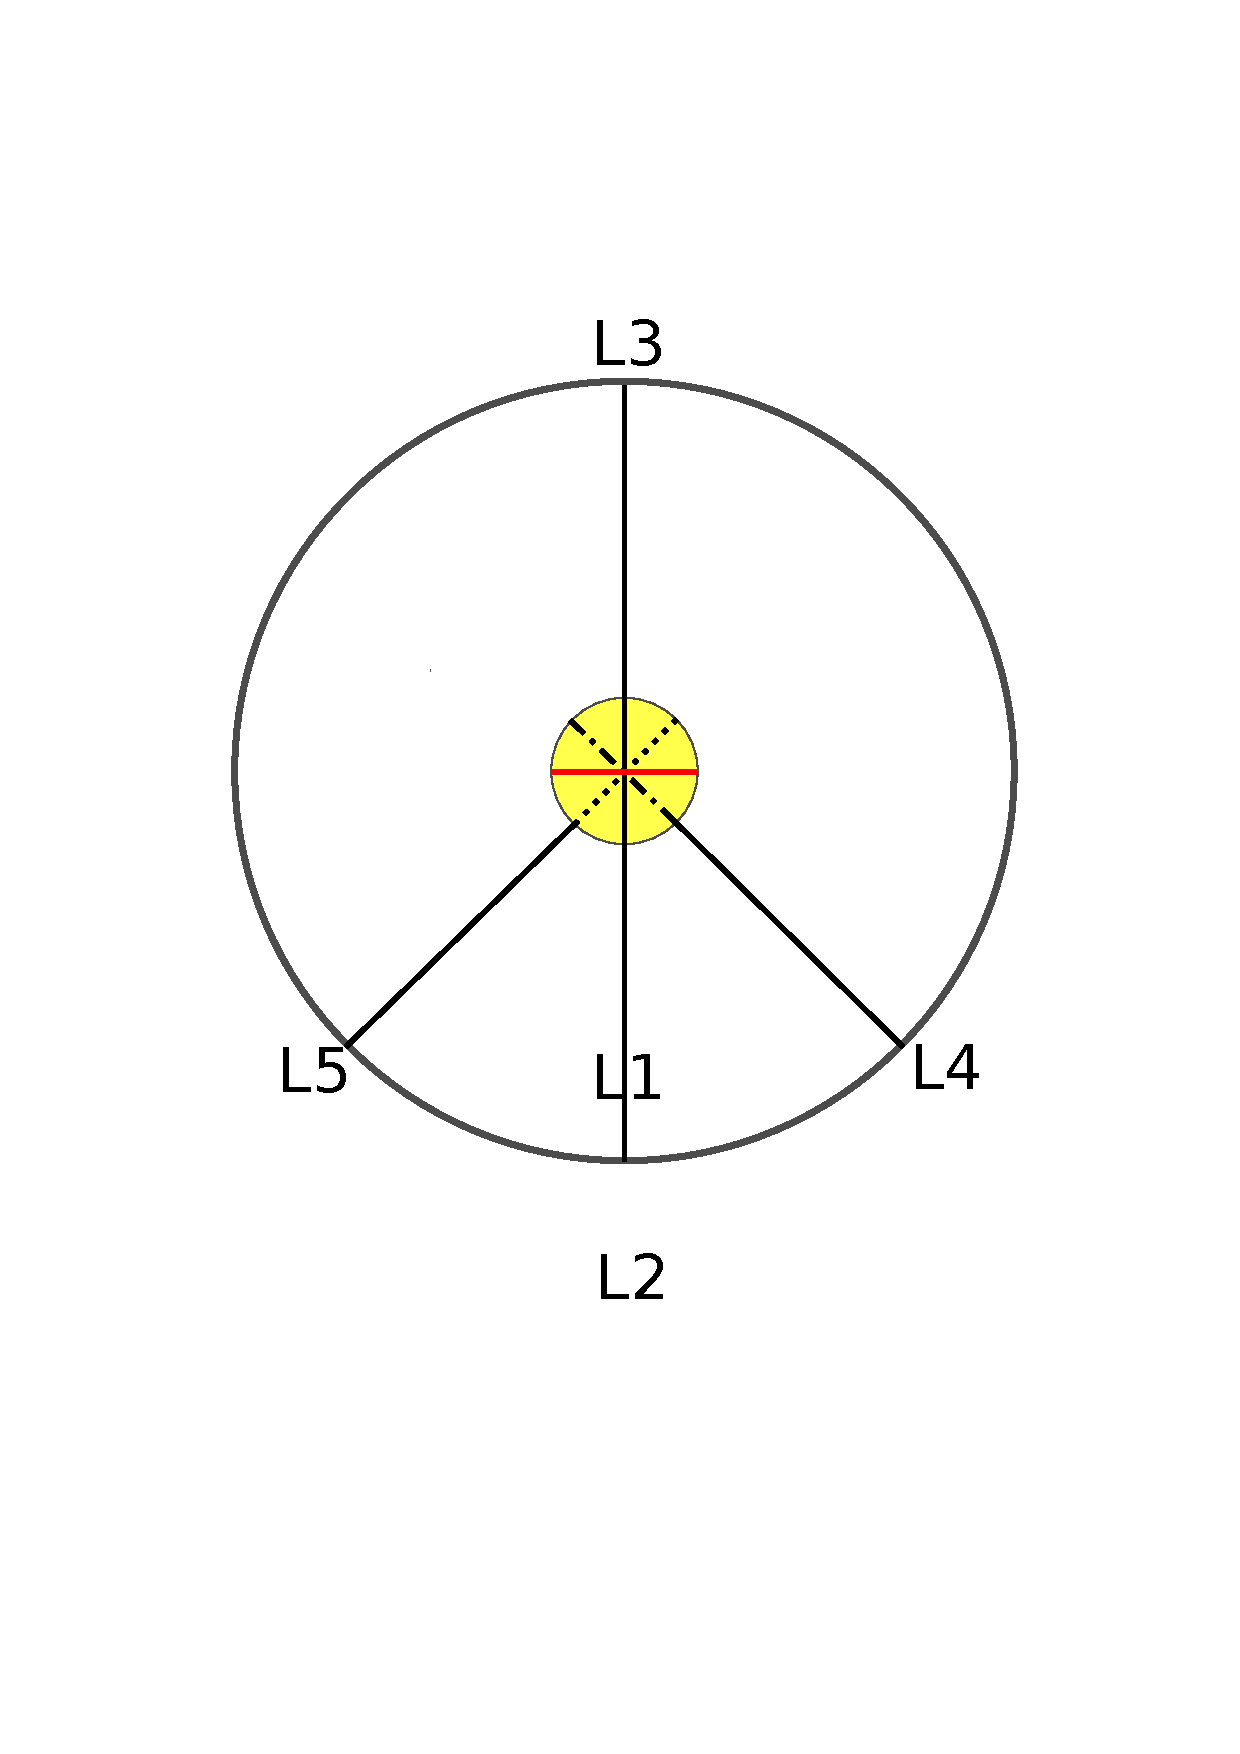
\includegraphics[trim={2cm 7cm 2cm 5cm}, clip, width=0.35\textwidth]{l1_l4_l5.pdf}
    \caption[Coverage of the solar surface with observations from various vantages.]{The Plane of projection of sun as seen from different vantages: solid red (observed from earth/L1), dotted black (observed from L4) and black dot-dashed (observed from L5). Figure is not to scale.}
    \label{fig:l1_l4_l5}
    \end{wrapfigure}
%%%%%%%%%%
    
Nevertheless, there are other unique advantages of such missions. L5 missions provide us the opportunity of predicting geo-effective eruptive events from the sun as it would be observing the regions of the sun turning towards the Earth. {\it Vigil} \citep{vigil} is a mission by ESA which is going to be placed in L5 for this very specific purpose. On the other hand, missions placed at L4 would be observing events on sun which would be more likely to end up being geo-effective. Materials ejected from west limb are more likely to follow the Parker spiral and hit Earth. Missions at L4 have the capability to provide us with high resolution remote observations before, during and after such events. There are various proposals of L4 missions already in discussion \citep{cho23}. The final advantage of continual observations from Earth/L1, L5 and L4 is illustrated in Fig.~\ref{fig:l1_l4_l5}. The plane of projection of solar disk from various perspective are shown in solid red (observed from Earth/L1), dotted black (observed from L4) and dot-dashed black (observed from L5). These combined observations would allow us to cover a significant portions of the far side of the sun. Currently the far side can only be observed during the flyby of orbiters {\it e.g. SO}, {\it STEREO-A}. It is safe to assume that the demographic of future space based solar missions would largely be shaped by the eventual outcome of current Lagrange point missions planned and under consideration. 

\noindent
{\bf Importance of current {\suit} flare observations and what are the future prospects?} {\suit} provides first full-disk solar imaging in all of the concerned pass bands. There are previous flare observations in some of the imaging channels {\it e.g.} NB3, NB4 and NB5 from {\it IRIS} and NB8 from {\it Hinode}/SOT, only in smaller spatial windows. One of the key disadvantage of smaller spatial windows is the possibility of missing events due to different pointing. {\suit}, equipped with its flare detection algorithm, has already observed several flares including various limb events. This provides us our first observation of off-limb flares in all these lines. A larger statistical study with such observations combined with EUV, SXR, HXR, H$\alpha$, and WL observations can provide us with more complete picture of how flare energy is deposited across various layers of the solar atmosphere.  

